\documentclass[../../../analisi-dei-requisiti.tex]{subfiles}

\begin{document}

\subsubsection{UUC12: Scelta noto o incognito}%
\label{subs:UUC12}

\begin{figure}[H]
  \centering
  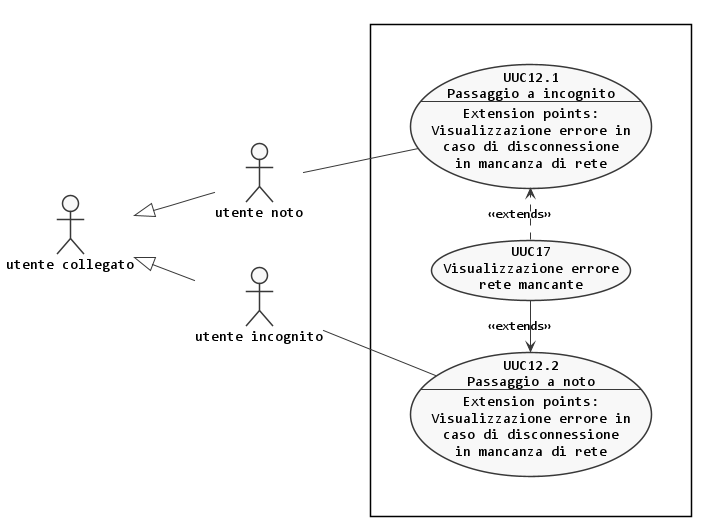
\includegraphics[width=150mm]{scelta-noto-o-incognito.png}
  \caption{UUC12: Scelta noto o incognito}%
  \label{fig:UUC12}
\end{figure}

\begin{description}
  \item[Caso d'uso:] UUC12;
  \item[Titolo:] Scelta noto o incognito;
  \item[Attori primari:] utente collegato, in particolare utente noto ed utente incognito;
  \item[Precondizione:] l'utente seleziona una o più organizzazioni da cui cambiare tipologia di presenza;
  \item[Postcondizione:] se l'utente era noto diventa incognito; vale anche il contrario;
  \item[Scenario principale:]
        \begin{enumerate}
          \item l'utente è collegato ad un'organizzazione in cui la sua presenza è nota; l'utente ha la possibilità di passare in modalità incognito;
          \item l'utente è collegato ad un'organizzazione in cui la sua presenza è incognita; l'utente ha la possibilità di passare in modalità nota.
        \end{enumerate}
  \item[Estensioni:]
        \begin{enumerate}
          \item se viene eseguita questa operazione in mancanza di rete, verrà visualizzato un errore~\ref{subs:UUC17}.
        \end{enumerate}
\end{description}

\subsubsection{UUC12.1: Passaggio a incognito}%
\label{subs:UUC12.1}
\begin{description}
  \item[Caso d'uso:] UUC12.1;
  \item[Titolo:] Passaggio a incognito;
  \item[Attori primari:] utente collegato, in particolare utente noto;
  \item[Precondizione:] l'utente deve essere collegato e noto;
  \item[Postcondizione:] l'utente è collegato ed incognito;
  \item[Scenario Principale:]
        \begin{enumerate}
          \item l'utente è noto in un'organizzazione e vuole diventare incognito: in questo modo la sua presenza è nota, ma non lo è la sua identità.
        \end{enumerate}
  \item[Estensioni:]
        \begin{enumerate}
          \item in caso di rete mancante, non possono essere eseguite queste operazioni e quindi verrà notificato un errore~\ref{subs:UUC17};
        \end{enumerate}
\end{description}

\subsubsection{UUC12.2: Passaggio a noto}%
\label{subs:UUC12.2}
\begin{description}
  \item[Caso d'uso:] UUC12.2;
  \item[Titolo:] Passaggio a noto;
  \item[Attori primari:] utente collegato, in particolare utente incognito;
  \item[Precondizione:] l'utente deve essere collegato ed incognito;
  \item[Postcondizione:] l'utente è collegato e noto;
  \item[Scenario Principale:]
        \begin{enumerate}
          \item l'utente è incognito in un'organizzazione e vuole diventare noto: in questo modo, sia la sua presenza che la sua identità sono note.
        \end{enumerate}
  \item[Estensioni:]
        \begin{enumerate}
          \item in caso di rete mancante, non possono essere eseguite queste operazioni e quindi verrà notificato un errore~\ref{subs:UUC17};
        \end{enumerate}
\end{description}


\end{document}
